\documentclass[a4paper,12pt]{article}


\usepackage{amsmath}
\usepackage[english]{babel}
\usepackage[utf8]{inputenc}
%\usepackage[ascii]{inputenc}
\usepackage{amssymb}
\usepackage{graphicx}
\usepackage{varioref}
%\usepackage[margin=.9in]{geometry}
\usepackage[a4paper, top=2cm, bottom=2cm, left=2.5cm, right=1cm]{geometry}
\usepackage{abstract}
\usepackage[T1]{fontenc}
%\usepackage{float}
\usepackage[english]{babel}
\usepackage{fancyhdr}		% for headers

%appendix
\usepackage[title,titletoc,toc]{appendix}

%***************** Packages for Graphics & Figures *******************%
\usepackage{graphicx} %%For loading graphic files
\graphicspath{ {images/} } %graphics path located inside image folder
%*******************************************************************%

\fancyhf{}
\fancyhead[l]{EE712 Embedded System Design Course Project Report, EE Dept, IIT Bombay, May,2016 (Course Instructor - Prof. P. C. Pandey)}
\fancyfoot[c]{\thepage}

\pagestyle{fancy}

% % convert plain page style to fancy on title page
\makeatletter
\let\ps@plain\ps@fancy 
\makeatother


\begin{document}
\begin{titlepage}

\end{titlepage}
%opening
\title
	{
		Programmable Noise Generator
	}
\author
	{
		Akshay Kumar Bajpai (143079003) akshaybajpai[at]ee.iitb.ac.in\\
		Piyush Manavar (153076006) piyush[at]ee.iitb.ac.in	\\
		Saurav Shandilya (153076004) shandilya[at]ee.iitb.ac.in\\
		Group: Monday-01
	}

\maketitle


\begin{abstract}
 	This projects aims at getting a programmable band limited noise by digital filtering white noise obtained by Pseudo Random Binary Sequence (PRBS) generator. PRBS is generated using 32 stage linear feedback shift registers (LFSR). The PRBS output spectrum approximates a white noise spectrum. The filter coefficients, of an 8-tap FIR filter to convert the white noise (PRBS output) to band limited noise, are obtained using MATLAB. Filtering is done by resistance-weighted op-amp based network for realizing a digital FIR filter from the shift register taps. Digital potentiometer (AD8403) has been used for getting variable resistors of summer circuit. The FFT spectrum of the PRBS and the output noise obtained are analyzed using a DSO and this matches the expected outcome. User interface is a python based GUI.

\end{abstract}


\section{Introduction}

Simple low-pass filtering of the output bit pattern of a PRBS generates band-limited white Gaussian noise, i.e., a noise voltage with a flat power spectrum up to some cutoff frequency. Alternatively, a weighted sum of the shift register contents (via a set of resistors) performs digital filtering, with the same result. Flat noise spectra out to several megahertz can easily be made this way. Such digitally synthesized analog noise sources have many advantages over purely analog techniques such as noise diodes or resistors.

A disadvantage of analog filtering is the need to readjust the filter cutoff if the clock frequency is changed by large factors. In situations where that is desirable, an elegant solution is provided by digital filtering, in this case performed by taking an analog weighted sum of successive output bits (non-recursive digital filtering). In, this way the effective filter cutoff frequency changes to match changes in the clock frequency. In addition, digital filtering lets you go to extremely low cutoff frequencies (fractions of a hertz) where analog filtering becomes awkward.

\section{Problem Statement}
To design a programmable(GUI controlled) noise generator using PRBS sequence utilizing a digital filter realized from an op-amp based summer circuit.

\section{Literature Review}

\subsection{Pseudo Random Binary Sequence}  
The chapter Digital meets Analog in \cite{aoe} mentions the generation of white noise using PRBS and filtering the output using resistors and op-amps. The project implementation is based on this idea. Programmable noise generator is achieved using linear feedback shift register (LFSR) (as shown in figure-\ref{fig:galois}) to generate the Pseudo Random Binary Sequence(PRBS). Shift register and XOR logic is used for generating PRBS\cite{lfsr_ti}. At every clock cycle, shift register advances the signal through the register from one bit to the next most-significant bit. Some of the outputs are tapped in XOR logic to form a feedback mechanism. LFSR is provided with an initial non-zero value and as operation of shift register is deterministic. XOR operation in feedback loop with some of the bits, generate values which are pseudo random in nature and will repeat the sequence eventually. \\
It is crucial to decide the bits which can used for generating feedback. These bits will plays a part into generating the delay after which sequence is repeated. The maximum number of conceivable states of an n-bit register is $L = 2^n$. However the state of all 0’s would get stuck in this circuit, since the XOR would regenerate a 0 at the input. Therefore an n-bit shift register, is called maximum-length LFSR if it is able to generate all possible sequence, which is $2^n-1$. Bits required for generating maximal-length LFSR is generated by solving primitive polynomial. \\
The arrangement of taps for feedback in an LFSR can be expressed in finite field arithmetic as a polynomial mod 2. This is called the feedback polynomial. The LFSR is maximal-length if the corresponding feedback polynomial is primitive. For polynomial to be primitive, following conditions are necessary:\\
1. The number of taps should be even.\\
2. The set of taps, taken all together, must be relatively prime. In other words, there must be no divisor other than 1 common to all taps.

We have used 32-bit shift register and primitive polynomial is $x^{32}+x^{30}+x^{26}+x^{25}+1$ \cite{lfsr_table}. Two commonly known techniques for generating LFSR are Fibonacci LFSR and Galois LFSR\cite{lfsr_wiki}. In Fibonacci LFSR rightmost bit of the LFSR is taken for output. The taps are XOR'd sequentially with the output bit and then fed back into the leftmost bit. The sequence of bits in the rightmost position is called the output stream. This techniques is also referred to as many-one or external gate configuration. In Galois LFSR, structure is altered to generate output same as Fibonacci LFSR but shifted in time. Bits that are not taps are shifted to right by one position. Bits that are tapped are XOR'd with the output bit before they are stored in the next position. The new output bit is the next input bit. The effect of this is that when the output bit is zero all the bits in the register shift to the right unchanged, and the input bit becomes zero. When the output bit is one, the bits in the tap positions all flip (if they are 0, they become 1, and if they are 1, they become 0), and then the entire register is shifted to the right and the input bit becomes 1. 32-bit Galois LFSR is shown in figure-\ref{fig:galois} The maximal length obtained for 32-bit register is 4294967295.

\begin{figure}[!ht]
	\centering
	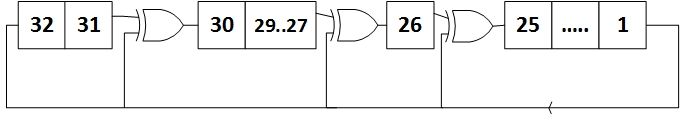
\includegraphics[scale=0.6]{galois.jpg}
	\caption{32-bit Galois LFSR with Tap position for maximal length}
	\label{fig:galois}
\end{figure}


\begin{figure}[!ht]
	\centering
	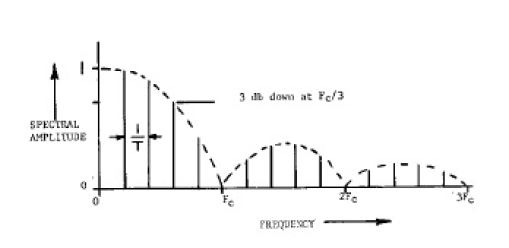
\includegraphics[scale=0.8]{PRS_fft}
	\caption{FFT for Pseudo Random Sequence}
	\label{fig:fft}
\end{figure}


\subsection{Analog noise generation from maximal-length sequences}
The output spectrum generated by maximal-length shift registers consists of noise extending from the repeat frequency of the entire sequence, $f_{clock}/L$, to the clock frequency and beyond. It is flat within $\pm0.1dB$ up to $12\%$ of the clock frequency ($f_{clock}$) , dropping rather rapidly beyond its $-3$ dB point of $44\%$ $f_{clock}$. The power spectrum is a set of equally spaced series of spikes (delta functions), beginning at the frequency at which the whole sequence repeats, $f_{clock}/L$, going up in frequency by equal intervals $f_{clock}/L$.\cite{aoe} The fact that the spectrum consists of a set of discrete spectral lines reflects the fact that the shift register sequence eventually (and periodically) repeats itself. It will look continuous for any measurement or application that takes less time than the cycle time of the register. The envelope of the spectrum of the unfiltered output is shown in figure-\ref{fig:fft}. The envelope is proportional to the square of $(sin x)/x$. Note the peculiar property that there is no noise power at the clock frequency or its harmonics.

\subsection{FILTER DESIGN FOR NOISE SHAPING}
\subsubsection{Digital Filtering}
   The digital filtering is performed by taking an analog weighted sum of successive output bits (non-recursive digital filtering). In order to perform a weighted sum of successive output bits simultaneously, we simply look at the various parallel outputs of the successive shift register bits using resistors of various values into an op-amp summing junction. For a low-pass filter the weights are proportional to the $(sin x / x)$. Note that some levels will have to be inverted, since the weights are of both signs. Since no capacitors are used in the scheme, the output waveform consists of a set of discrete output voltages. We wrote a simple MATLAB program to determine the values of the resistances.\\
   
   \begin{figure}[!ht]
   	\centering
   	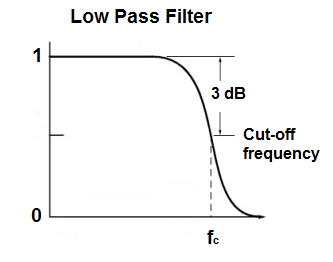
\includegraphics[scale=0.8]{lp_filter}
   	\caption{Low Pass Filter Response}
   	\label{fig:lp}
   \end{figure}
   The resistances corresponding to the particular low pass filter are determined for white noise using the FIR filter design theory. Key idea is to start with desired frequency response and then take its inverse FFT for finding resistance values.
   
\subsubsection{Basic Properties of FIR Digital Filters}
   Digital FIR (finite impulse response) filters cannot be derived from analog filters, since rational analog filter cannot have a finite impulse response. In many digital signal processing applications, FIR filters are preferred over their IIR counterparts. The main advantages of the FIR filter designs over their IIR equivalents are the following:
   \begin{itemize}
   	\item FIR filters with exactly linear phase can easily be designed. This simplifies the approximation problem, in many cases, when one is only interested in designing of a filter that approximates an arbitrary magnitude response. Linear phase filters are important for applications where frequency dispersion due to nonlinear phase is harmful e.g. speech processing and data transmission.
   	\item There are computationally efficient realizations for implementing FIR filters. These include both non-recursive and recursive realizations.
   	\item FIR filters realized non-recursively are inherently stable and free of limit cycle oscillations when implemented on a finite-word length digital system.
   	\item Excellent design methods are available for various kinds of FIR filters with arbitrary specifications.
   	\item The output noise due to multiplication round off errors in an FIR filter is usually very low and the sensitivity to variations in the filter coefficients is also low. 
   \end{itemize}

\subsubsection{Frequency Response of Linear Phase FIR Digital Filters}
   One of the simplest types of filters that we can design is an FIR filter with linear phase. Also, only FIR filters can be designed to have linear phase response. It can be shown also that IIR filters cannot have linear phase.
   
\subsubsection{Uniform Frequency-Sampling Method}
   The frequency sampling method for FIR filter design is basically the technique we shall be using to generate the filter weights. Here, we specify the desired frequency response at a set of equally spaced frequencies. We solve for the unit sample response $h(n)$ of the FIR filter from these equally spaced specification.\cite{dsp}\\
   We shall begin with the frequency response of the FIR filter
   
   \begin{equation}  
   \begin{aligned}
  y(n) &= \sum_{k=0}^{M-1}h(k)x(n-k)\\
   \end{aligned} 
   \end{equation}
     
   \begin{equation}  
   \begin{aligned}
  H(e^{iw}) = \sum_{n=0}^{M-1}h(n)e^{-iwn}\\
   \end{aligned} 
   \end{equation}
     
   If the frequency response of the filter is specified at the frequencies
   \begin{equation}  
      \begin{aligned}
     w_k = 2\pi k/M\\
      \end{aligned} 
      \end{equation}
   
   then we can obtain
   \begin{equation}  
         \begin{aligned}
        H(e^{iw}) = H(w_k) = H(2\pi k/M) = H(k)\\
         \end{aligned} 
         \end{equation}
   	
   and
   \begin{equation}  
            \begin{aligned}
           H(k) = \sum_{n=0}^{M-1}h(n)e^{-i2\pi nk/M}          	\hspace{32pt}   for\hspace{2pt} k=0,1,2......M-1\\
            \end{aligned} 
            \end{equation}
  
      
   The above expression of $H(k)$ is nothing but the DFT of $h(n)$ . Thus $h(n)$ may be visualized as the inverse DFT of $H(k)$ . Once we obtain the above filter coefficients, then it is easy to design filter as the resistances that we use in digital filtering are the ratios of op-amp’s feedback resistor to the real part of $h(n)$ coefficients.
   

\section{Block Diagram}

\begin{figure}[!ht]
	\centering
	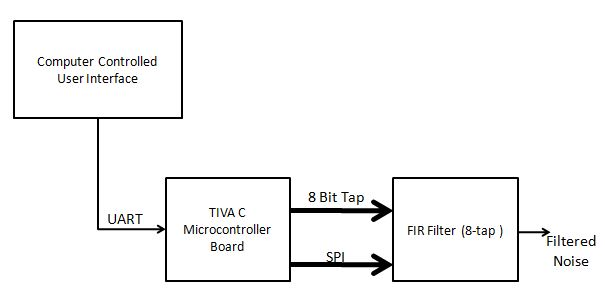
\includegraphics[scale=0.8]{block_dia}
	\caption{Block Diagram}
	\label{fig:block}
\end{figure}

System comprises of a python based graphical user interface running on a PC. User can control cut-off frequency of FIR filter and clock frequency of LFSR. User Interface transmits data serially through UART to TIVA C series microcontroller\cite{tiva}. Microcontroller generates the filter coefficient values and accordingly controls digital potentiometer via SPI communication channel. We have used two digital potentiometers(AD8403), each having four on-chip variable resistors. Hence we can realize a 8-tap programmable FIR filter which gives a band limited noise at its output.
   
\section{Components Used}
\begin{enumerate}
	\item TIVA C series Launchpad - TM4C123GH6PM
	\item Digital Potentiometer(R$max$100K) - AD8403 \cite{dpot_datasheet} (02)
	\item LM 324 (01)
	\item LM 741 (01)
	\item Bread Board (01)
	\item Power Supply – Aplab LQ6324 (01)
	\item DSO - Aplab D37200B4 (01)
	 (01)
	\item Wires and Probes
\end{enumerate}

\section{Circuit Diagram}
Circuit diagram is shown below
\begin{figure}[!ht]
	\centering
	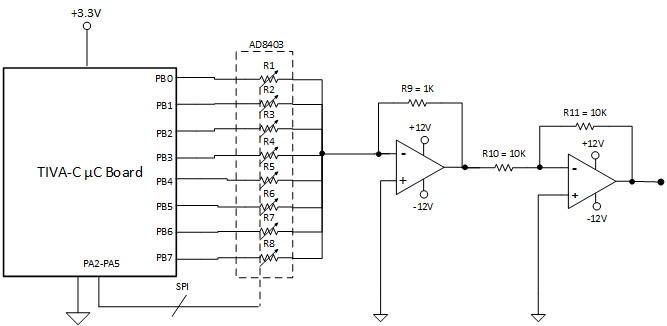
\includegraphics[scale=0.8]{circuit-dig}
	\caption{Circuit diagram for FIR Filtering}
	\label{fig:circuit}
\end{figure}

\section{Design of resistors for the op-amp summer}
Refer to the op-amp summer block diagram given in figure-\ref{fig:circuit}. We find 8 tap FIR filter coefficients in MATLAB by taking Inverse FFT of desired filter response(low pass filter) as described in section 3.3.4. Then resistances that we use in digital filtering are the ratios of op-amp’s feedback resistor to the real part of filter coefficients. Second op-amp is provided to just make overall gain positive.\\
Here we have chosen: \\[1mm]
$R9 = 1 K\Omega$	\\
$R10 = 10 K\Omega$	\\	
$R11 = 10 K\Omega$	\\


So $R1$ to $R8$ were found using R9 as described above which depend upon the cut off frequency of the desired low pass filter.

\begin{figure}[!ht]
	\centering
	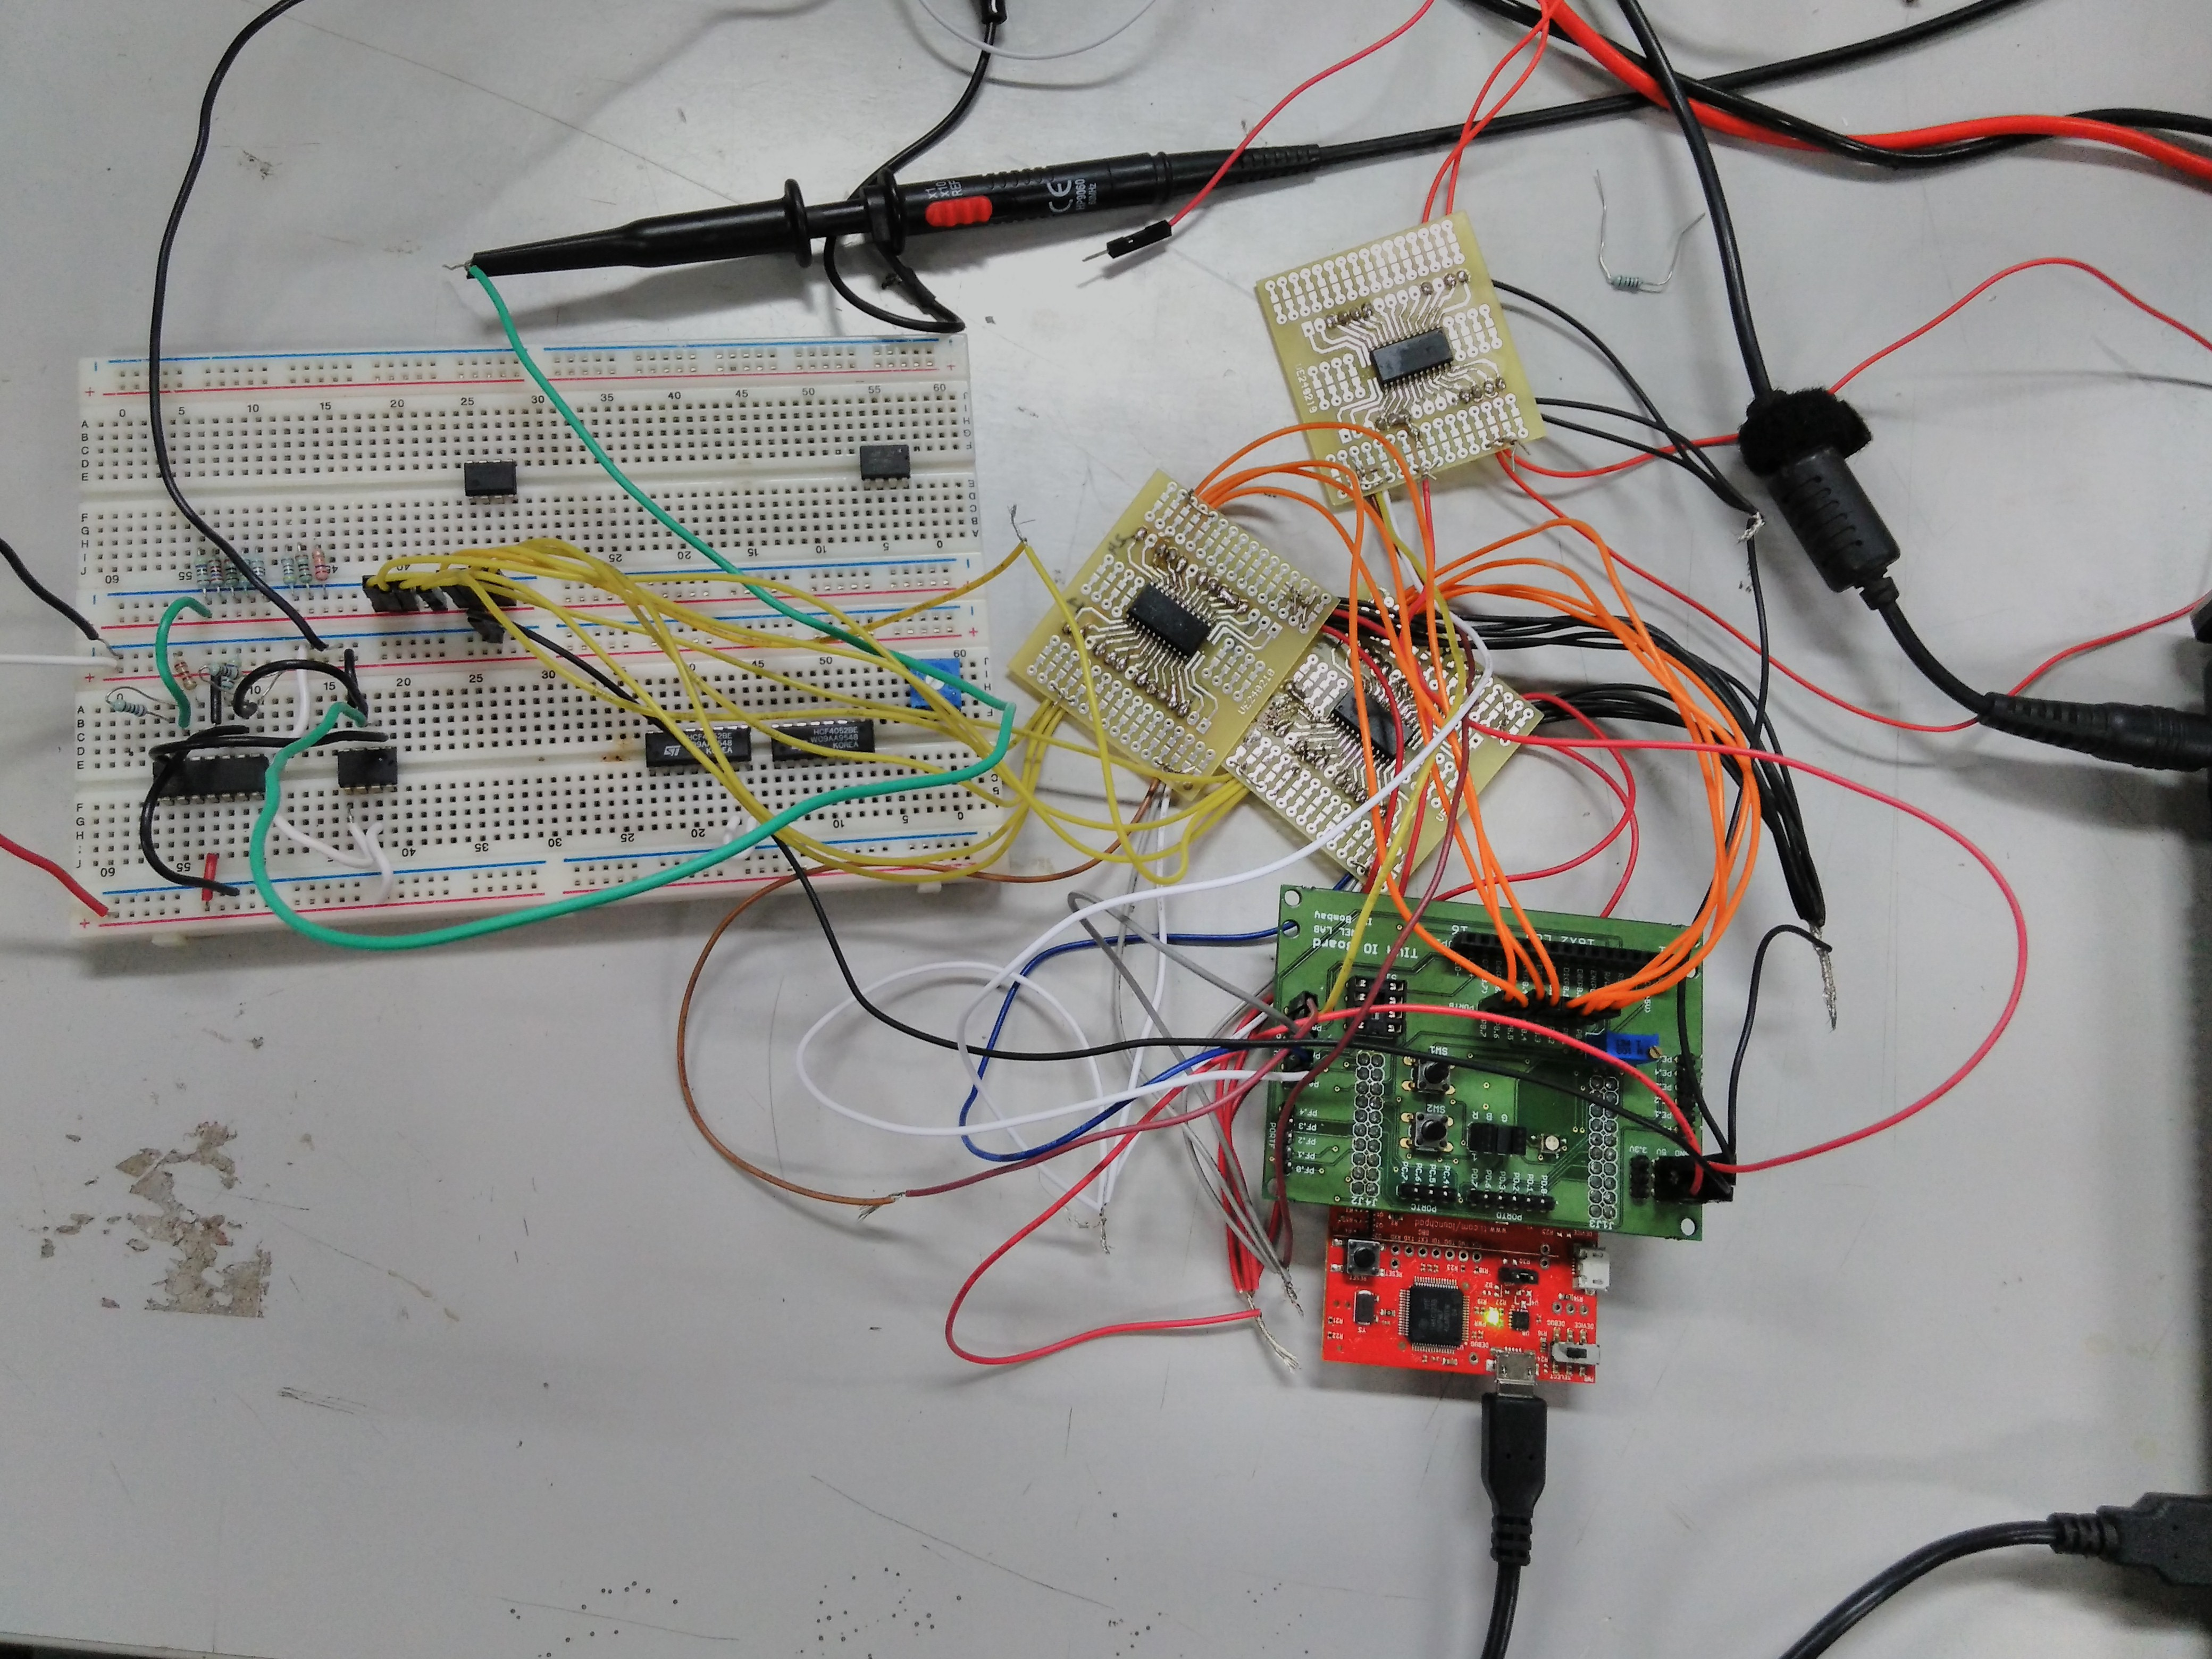
\includegraphics[width=\linewidth,height=11cm]{setup.jpg}
	\caption{Our system setup}
	\label{fig:setup}
\end{figure}

\begin{figure}[!ht]
	\centering
	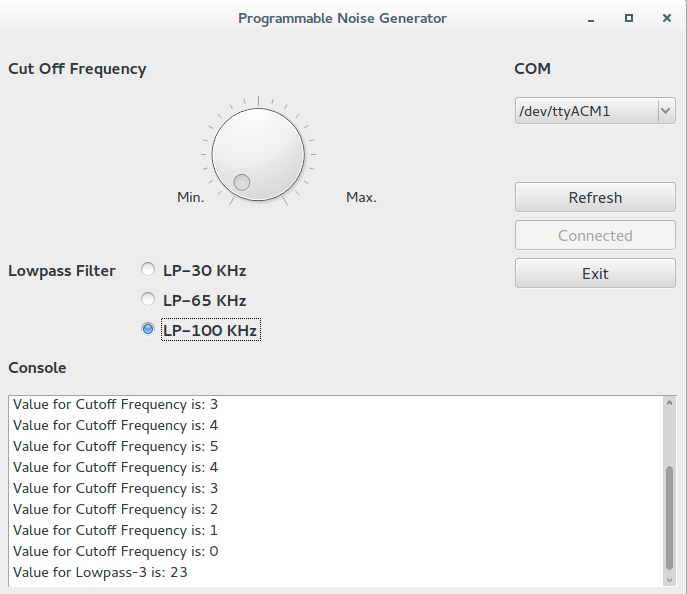
\includegraphics[width=13cm,height=11cm]{gui.png}
	\caption{Python based GUI}
	\label{fig:gui}
\end{figure}


\section{Test Results}
In this section we present our setup, GUI and various waveforms which we captured during test of the system. All waveforms were captured from DSO and controls were given from a python based GUI to generate these waveforms.

\begin{figure}[!ht]
	\centering
	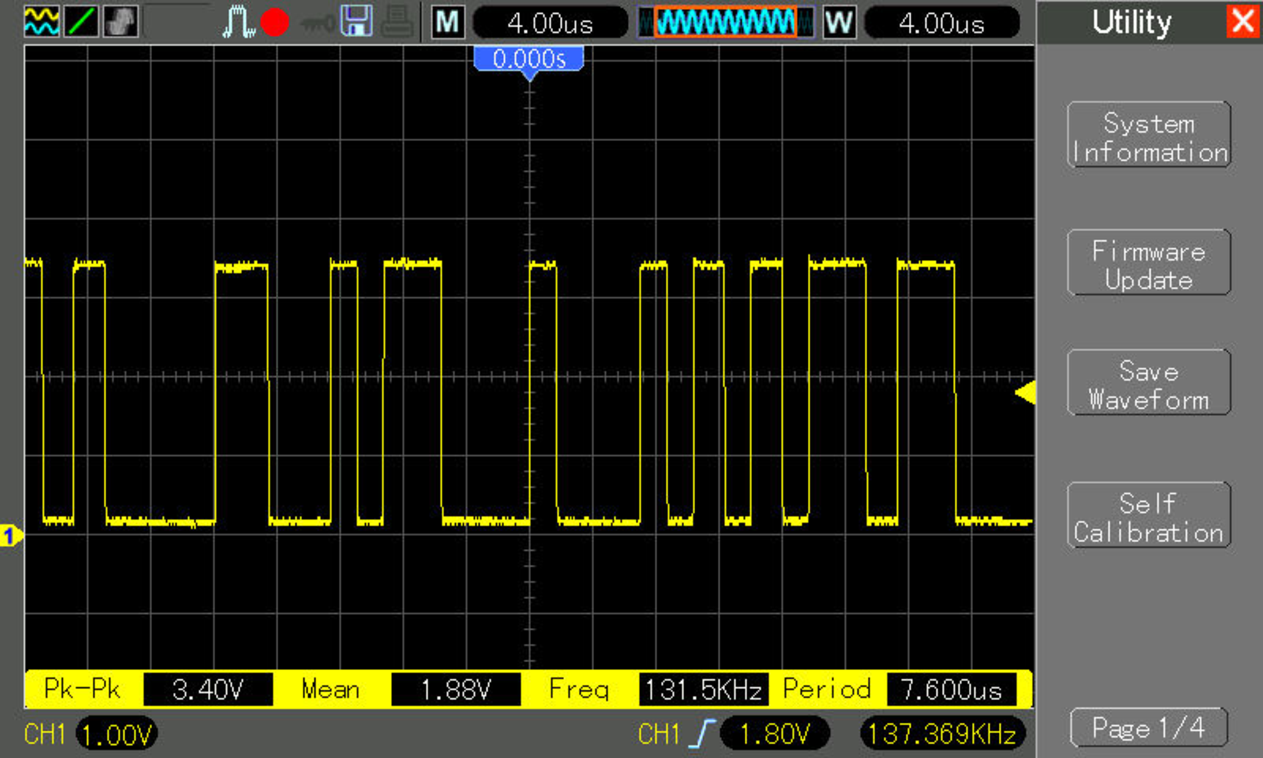
\includegraphics[width=\linewidth,height=11cm]{pic_488_2.pdf}
	\caption{Time domain PRBS waveform at $f_{clk} = 520Khz$}
	\label{fig:result-2}
\end{figure}

\begin{figure}[!ht]
	\centering
	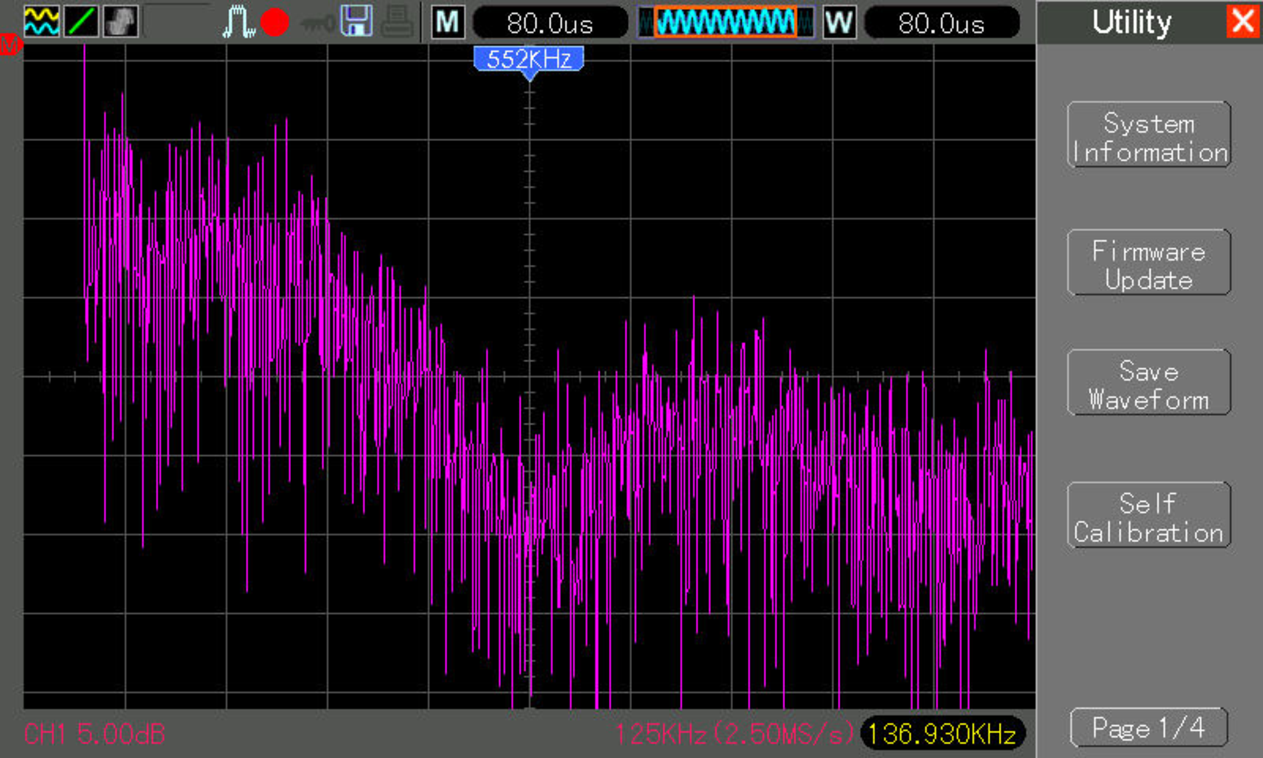
\includegraphics[width=\linewidth,height=11cm]{pic_488_3.pdf}
	\caption{Frequency domain PRBS waveform at $f_{clk} = 520Khz$}
		\label{fig:result-3}
\end{figure}



\begin{figure}[!ht]
	\centering
	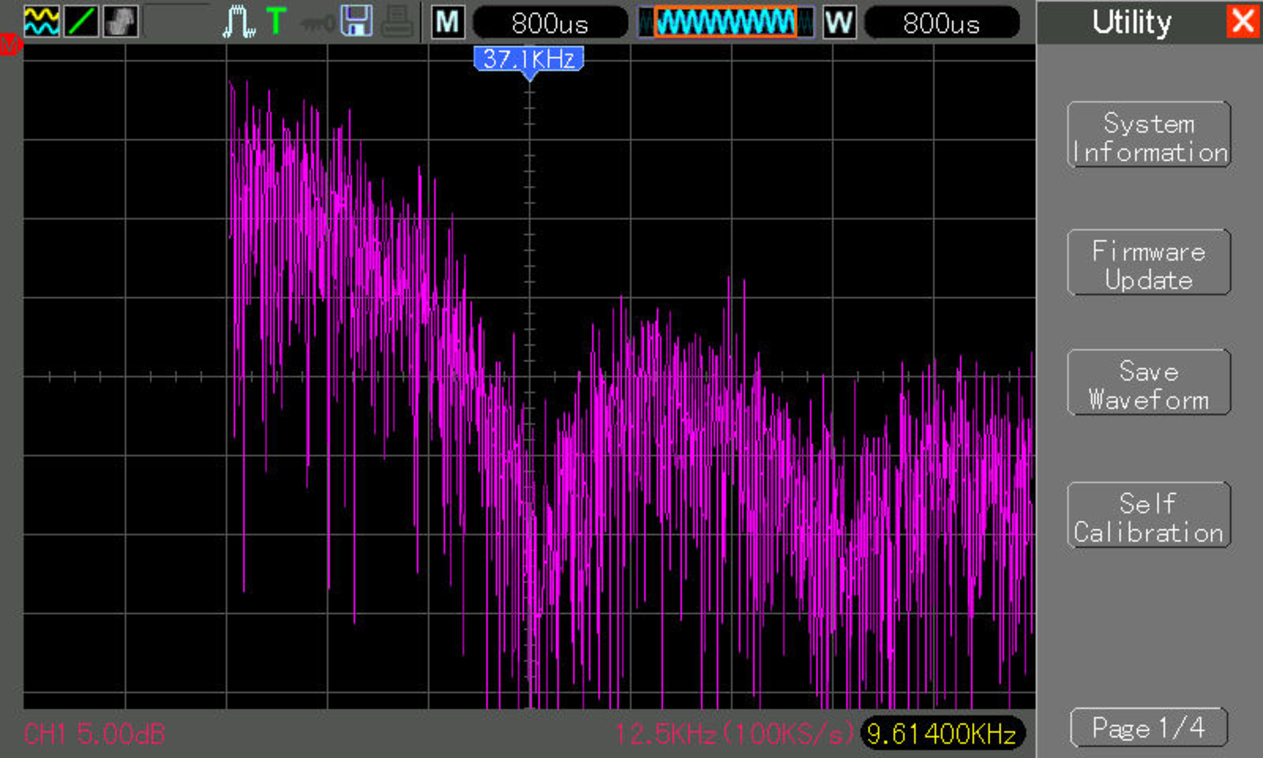
\includegraphics[width=\linewidth,height=11cm]{pic_489_1.pdf}
	\caption{Frequency domain PRBS waveform at $f_{clk} = 45Khz$}
		\label{fig:result-4}
\end{figure}

\begin{figure}[!ht]
	\centering
	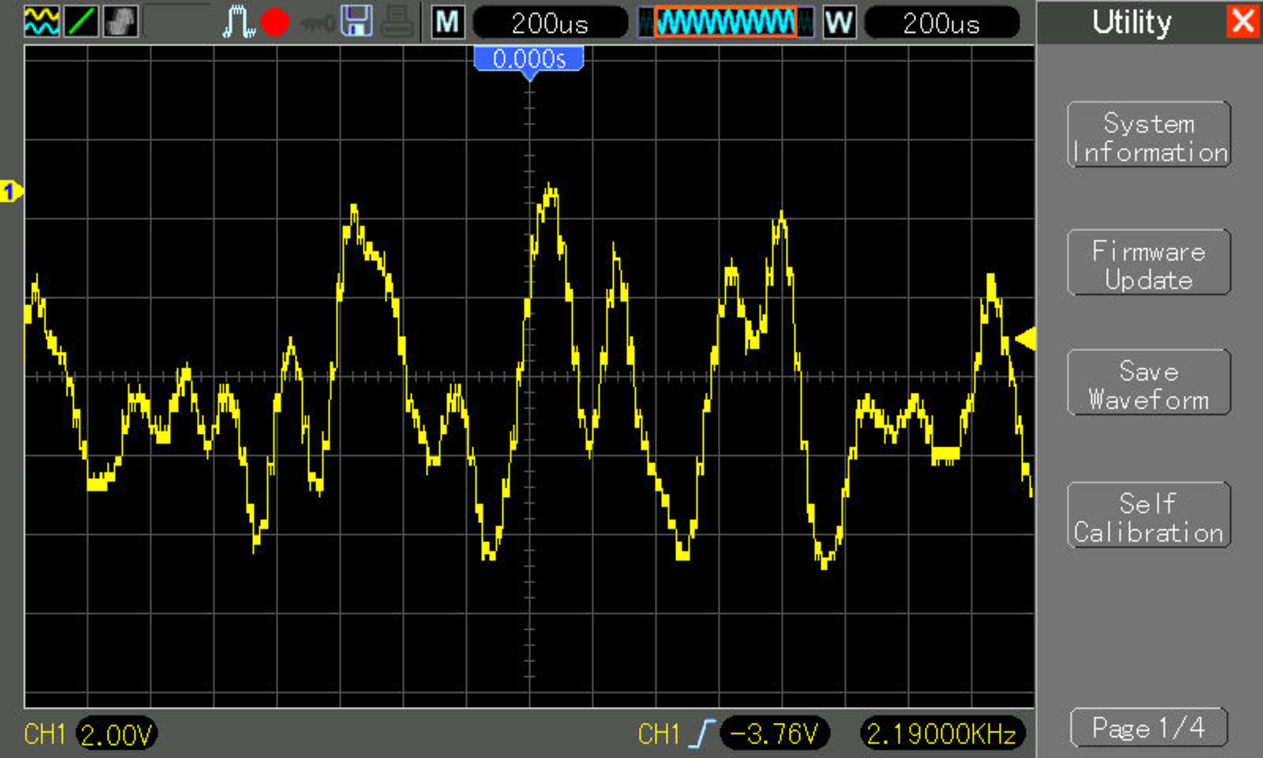
\includegraphics[width=\linewidth,height=11cm]{pic_488_1.pdf}
	\caption{Time domain FIR filtered waveform at $f_{clk} = 45Khz$}
	\label{fig:result-1}	
\end{figure}

\begin{figure}[!ht]
	\centering
	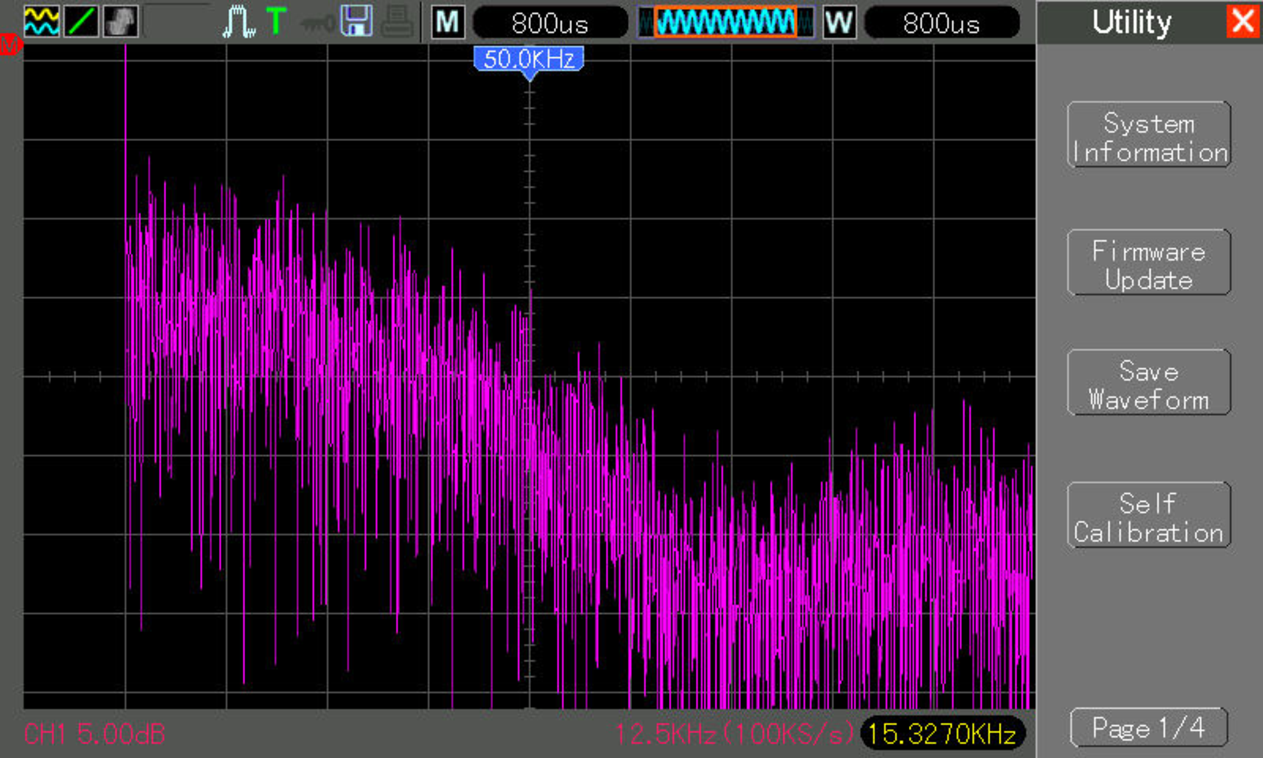
\includegraphics[width=\linewidth,height=11cm]{pic_490_1.pdf}
	\caption{Frequency domain FIR filtered waveform at $f_{clk} = 45Khz$}
	\label{fig:result-7}
\end{figure}

\begin{figure}[!ht]
	\centering
	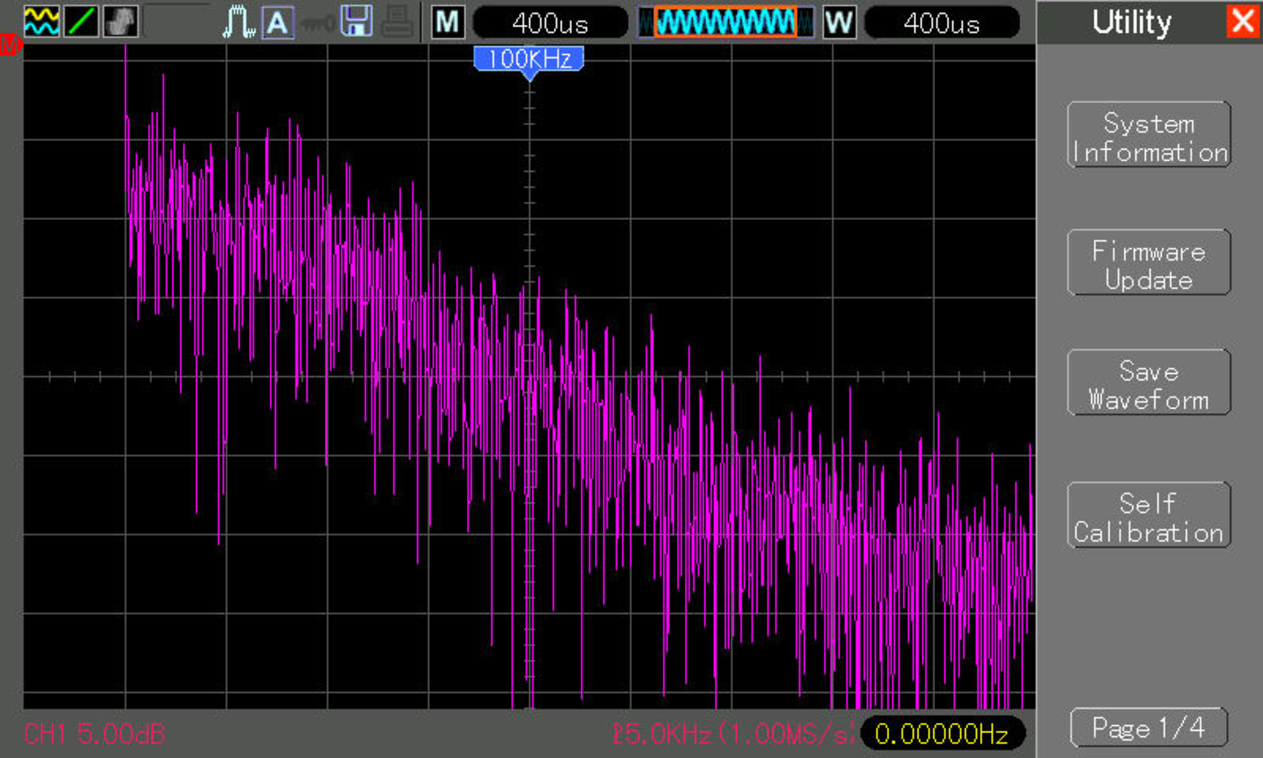
\includegraphics[width=\linewidth,height=11cm]{pic_489_3.pdf}
	\caption{Frequency domain FIR filtered waveform at $f_{clk} = 520Khz$}
	\label{fig:result-6}
\end{figure}

\newpage	
\section{Discussion of the Results}
Various waveforms and results obtained are as expected theoretically. The cut off frequency of PRBS decreases with decreasing clock rate of LFSR. In addition, low pass filter was also limiting the PRBS bandwidth hence producing the desired band limited noise.  

%\section{Challenges}
\section{Conclusion}
We have obtained White noise using 32-bit maximal length PRBS from TIVA microcontroller. The White noise output is filtered by using an 8-tap FIR filter. This filter has been realized using a set of resistors (potentiometers) and an op-amp. The spectrum of PRBS output and the filtered output have been analyzed in FFT mode of DSO. It has been verified that the envelope of the spectrum of the PRBS output is proportional to the square of $(sin x)/x$. The spectrum of the filtered output is band limited to certain cut-off frequency decided by digital filter. Python GUI was used to control cut-off frequency of band limited noise. In future, other filters such as band pass, high pass etc. may also be included.


\bibliographystyle{unsrt}
\bibliography{EE712_reference}


\end{document}
